\documentclass{cshwk}

\title{HW \#3, Chapter 3}

\begin{document}

\maketitle

\section*{Chapter 3, P40}

Consider Figure~\ref{fig:tcp-reno}. Assuming TCP Reno is the protocol experiencing the behavior shown above, answer the following questions. In all cases, you should provide a short discussion justifying your answer.

\begin{figure}[htbp]
    \centering
    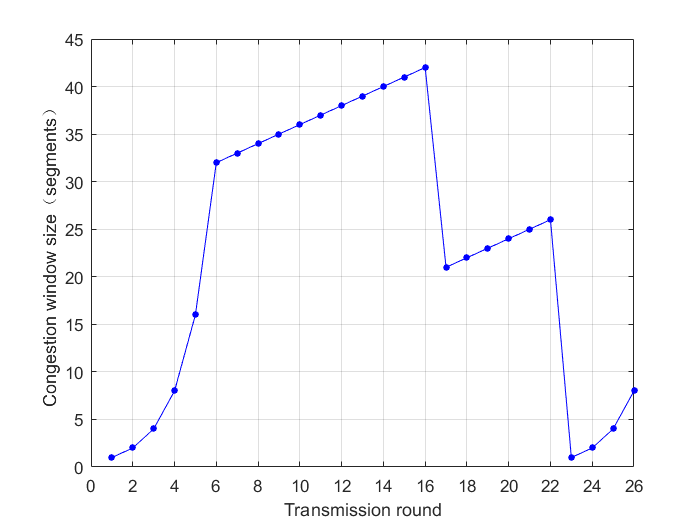
\includegraphics[width=0.8\textwidth]{hw3-5-1.png}
    \caption{TCP Reno}
    \label{fig:tcp-reno}
\end{figure}

\begin{enumerate}
    \item Identify the intervals of time when TCP slow start is operating.
    \item Identify the intervals of time when TCP congestion avoidance is operating.
    \item After the 16th transmission round, is segment loss detected by a triple duplicate ACK or by a timeout?
    \item After the 22nd transmission round, is segment loss detected by a triple duplicate ACK or by a timeout?
    \item What is the initial value of \texttt{ssthresh} at the first transmission round?
    \item What is the value of \texttt{ssthresh} at the 18th transmission round?
    \item What is the value of \texttt{ssthresh} at the 24th transmission round?
    \item During what transmission round is the 70th segment sent?
    \item Assuming a packet loss is detected after the 26th round by the receipt of a triple duplicate ACK, what will be the values of the congestion window size and of \texttt{ssthresh}?
    \item Suppose TCP Tahoe is used (instead of TCP Reno), and assume that triple duplicate ACKs are received at the 16th round. What are the \texttt{ssthresh} and the congestion window size at the 19th round?
    \item Again suppose TCP Tahoe is used, and there is a timeout event at the 22nd round. How many packets have been sent out from the 17th round till 22nd round, inclusive?
\end{enumerate}

\section*{Solutions}

\paragraph{1.} Slow start is observed from \textbf{round 1 to round 6}. The congestion window increases exponentially, which is a characteristic of the slow start phase.

\paragraph{2.} Congestion avoidance is active after slow start until segment loss is detected. This can be seen from around \textbf{round 7 to round 16}, where the increase in the congestion window becomes linear.

\paragraph{3.} At round 16, the graph shows a sharp drop in the congestion window. This indicates a segment loss detected by either a timeout or a triple duplicate ACK. Since it didn't drop to 1, \textbf{the sharp drop suggests a loss detected by a triple duplicate ACK.}

\paragraph{4.} After round 22, another sharp drop is visible, indicating segment loss. Given the behavior of droping to 1, \textbf{the loss is detected by a timeout.}

\paragraph{5.} \textbf{The initial value of \texttt{ssthresh} is 32}, as shown in the round 6 where reached 32 and the slow start phase ends.

\paragraph{6.} At the 18th round, \textbf{the value of \texttt{ssthresh} is 21}. The value is halved from the previous \texttt{cwnd} value of 42, which was set after the loss event at round 16.

\paragraph{7.} After the second loss event around round 22, ssthresh is halved again. Just before round 22, cwnd was around 26, \textbf{so ssthresh would now be about 13 segments.}

\paragraph{8.} \textbf{The 70th segment would likely be transmitted sometime before round 7}, during congestion avoidance.

\paragraph{9.} After the loss event at round 26, the congestion window is reduced halved to 4, and \texttt{ssthresh} is set also to 4.

\paragraph{10.} In TCP Tahoe, after a triple duplicate ACK, \texttt{ssthresh} is set to half of the current congestion window size, \textbf{which is 21}. So, \texttt{ssthresh} and the \textbf{congestion window size will be set to 1.}

\paragraph{11.} In TCP Tahoe, the congestion window is set to 1 and \texttt{ssthresh} is set to half of the current congestion window size, which is 21. So, \texttt{ssthresh} and the \textbf{congestion window size will be set to 1.} The packets sent from the 17th round to the 22nd round, inclusive, will be $1+2+4+8+16+21(\textbf{22rd, Timeout happened}) = \mathbf{52}$ packets

\end{document}